\documentclass[tikz,border=4pt]{standalone}
\usepackage[T1]{fontenc}\usepackage{helvet}\renewcommand{\familydefault}{\sfdefault}
\usepackage{xcolor}
\usetikzlibrary{arrows.meta,shapes,positioning,fit,backgrounds}
\definecolor{rscblue}{RGB}{0,83,156}\definecolor{rscgold}{RGB}{200,155,0}
\definecolor{cream}{RGB}{222,217,201}\definecolor{ddgray}{RGB}{88,100,112}
\newcommand{\logS}{\ensuremath{\log S}}
\begin{document}
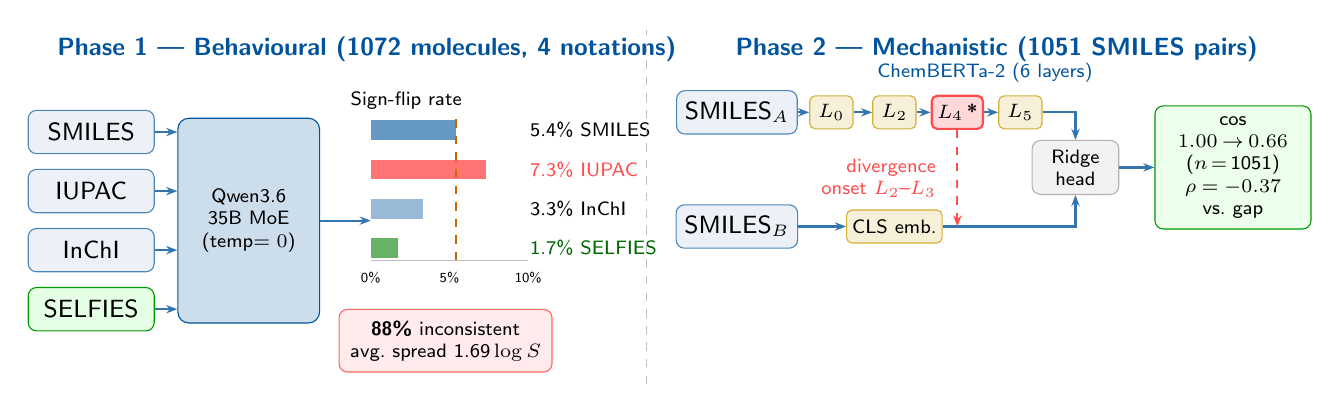
\begin{tikzpicture}[font=\sffamily\small,
  box/.style={draw=rscblue!70, rounded corners=3pt, fill=rscblue!8,
              minimum width=1.6cm, minimum height=0.55cm, align=center,
              inner sep=3pt},
  arrow/.style={-{Stealth[length=4pt]}, thick, color=rscblue!80},
  layerbox/.style={draw=rscgold!80, fill=rscgold!15, rounded corners=2pt,
                   minimum width=0.55cm, minimum height=0.42cm, align=center,
                   inner sep=2pt, font=\sffamily\scriptsize},
  bestlayer/.style={draw=red!70, fill=red!15, rounded corners=2pt,
                    minimum width=0.55cm, minimum height=0.42cm, align=center,
                    inner sep=2pt, font=\sffamily\scriptsize\bfseries, line width=0.8pt}]

%% ---- LEFT PANEL: Phase 1 overview ----
\node[font=\sffamily\bfseries\small, color=rscblue] at (0, 2.55) {Phase 1 — Behavioural (1072 molecules, 4 notations)};

% Notation boxes feeding into LLM
\node[box] (smiles)  at (-3.5, 1.5) {SMILES};
\node[box] (iupac)   at (-3.5, 0.75) {IUPAC};
\node[box] (inchi)   at (-3.5, 0.0)  {InChI};
\node[box,fill=green!10,draw=green!60!black] (selfies) at (-3.5,-0.75) {SELFIES};

% LLM box
\node[draw=rscblue, fill=rscblue!20, rounded corners=4pt,
      minimum width=1.8cm, minimum height=2.6cm, align=center,
      font=\sffamily\scriptsize] (llm) at (-1.5, 0.375) {Qwen3.6\\35B MoE\\(temp$=0$)};

\draw[arrow] (smiles.east)  -- (llm.west|-smiles.east);
\draw[arrow] (iupac.east)   -- (llm.west|-iupac.east);
\draw[arrow] (inchi.east)   -- (llm.west|-inchi.east);
\draw[arrow] (selfies.east) -- (llm.west|-selfies.east);

% Results: sign-flip bar chart (scale: 1% = 0.20 width)
\node[font=\sffamily\scriptsize, align=center] at (0.5, 1.9) {Sign-flip rate};
% bars
\fill[rscblue!60]   (0.05,  1.4) rectangle (0.05+1.08, 1.65);  % SMILES 5.4%
\fill[red!55]        (0.05,  0.9) rectangle (0.05+1.46, 1.15);  % IUPAC  7.3% (worst)
\fill[rscblue!40]   (0.05,  0.4) rectangle (0.05+0.66, 0.65);  % InChI  3.3%
\fill[green!50!black!60] (0.05, -0.1) rectangle (0.05+0.34, 0.15); % SELFIES 1.7%

% x-axis tick labels (0%, 5%, 10%)
\node[font=\sffamily\tiny, anchor=north] at (0.05,       -0.15) {0\%};
\node[font=\sffamily\tiny, anchor=north] at (0.05+1.00,  -0.15) {5\%};
\node[font=\sffamily\tiny, anchor=north] at (0.05+2.00,  -0.15) {10\%};
\draw[gray!50, line width=0.3pt] (0.05, -0.13) -- (0.05+2.00, -0.13);

% SMILES baseline dashed reference line at 5.4% (x = 0.05 + 1.08)
\draw[dashed, orange!80!black, line width=0.7pt]
  (0.05+1.08, -0.13) -- (0.05+1.08, 1.75);
% no separate label needed: bar already reads "5.4% SMILES" and dashed line is self-evident

% bar labels
\node[font=\sffamily\scriptsize, anchor=west] at (1.95, 1.525) {5.4\% {\scriptsize SMILES}};
\node[font=\sffamily\scriptsize, color=red!70, anchor=west] at (1.95, 1.025) {7.3\% {\scriptsize IUPAC}};
\node[font=\sffamily\scriptsize, anchor=west] at (1.95, 0.525) {3.3\% {\scriptsize InChI}};
\node[font=\sffamily\scriptsize, color=green!40!black, anchor=west] at (1.95, 0.025) {1.7\% {\scriptsize SELFIES}};

\draw[arrow] (llm.east) -- (0.05, 0.375);   % reach bar-chart left edge

% 95% inconsistency callout
\node[draw=red!60, fill=red!8, rounded corners=3pt, font=\sffamily\scriptsize,
      align=center, inner sep=4pt] at (1.0,-1.15)
      {\textbf{88\%} inconsistent\\avg.\ spread 1.69\,$\log S$};

%% ---- DIVIDER ----
\draw[dashed, gray!50, line width=0.6pt] (3.55, -1.7) -- (3.55, 2.8);

%% ---- RIGHT PANEL: Phase 2 overview ----
% Symmetric funnel layout: L5 drops into ridge.north, CLS rises into ridge.south.
% Result box to the RIGHT of Ridge head → no path collision.
\node[font=\sffamily\bfseries\small, color=rscblue] at (8.00, 2.55)
  {Phase 2 — Mechanistic (1051 SMILES pairs)};
\node[font=\sffamily\scriptsize, color=rscblue] at (7.85, 2.25)
  {ChemBERTa-2 (6 layers)};

% ---- Top rail: SMILES_A → L0 → L2 → L4* → L5 ----
\node[box, minimum width=1.3cm] (smiA) at (4.70, 1.75) {SMILES$_A$};
\node[layerbox] (L0) at (5.90, 1.75) {$L_0$};
\node[layerbox] (L2) at (6.70, 1.75) {$L_2$};
\node[bestlayer] (L4) at (7.50, 1.75) {$L_4$\,\textbf{*}};
\node[layerbox] (L5) at (8.30, 1.75) {$L_5$};

\draw[arrow] (smiA.east) -- (L0.west);
\draw[arrow] (L0.east)   -- (L2.west);
\draw[arrow] (L2.east)   -- (L4.west);
\draw[arrow] (L4.east)   -- (L5.west);

% ---- Bottom rail: SMILES_B → CLS emb. ----
\node[box, minimum width=1.3cm] (smiB) at (4.70, 0.30) {SMILES$_B$};
\node[layerbox] (L6) at (6.70, 0.30) {CLS emb.};
\draw[arrow] (smiB.east) -- (L6.west);

% ---- Ridge head: L5 enters from top, CLS enters from bottom (symmetric) ----
\node[draw=gray!60, fill=gray!10, rounded corners=3pt,
      minimum width=1.1cm, minimum height=0.5cm, align=center,
      font=\sffamily\scriptsize] (ridge) at (9.00, 1.05) {Ridge\\head};

% L5  → ridge.north:  corner at (9.00, 1.75), then drop
\draw[arrow] (L5.east) -| (ridge.north);
% CLS → ridge.south:  corner at (9.00, 0.30), then rise  ← symmetric to L5
\draw[arrow] (L6.east) -| (ridge.south);

% ---- Replacement annotation ----
\draw[-{Stealth[length=4pt]}, red!70, thick, dashed]
  (L4.south) -- (L4.south |- L6.east)
  node[midway, left=4pt, anchor=east, font=\sffamily\scriptsize,
       color=red!70, align=right] {divergence\\onset $L_2$--$L_3$};

% ---- Result box: to the RIGHT of Ridge head (no downward-path conflict) ----
\node[draw=green!60!black, fill=green!8, rounded corners=3pt,
      font=\sffamily\scriptsize, align=center, inner sep=4pt,
      text width=1.7cm] (result) at (11.00, 1.05)
      {cos $1.00\!\to\!0.66$\\($n$\,=\,1051)\\$\rho\!=\!-0.37$ vs.\ gap};
\draw[arrow] (ridge.east) -- (result.west);

\end{tikzpicture}
\end{document}
